\documentclass[10pt,aspectratio=169]{beamer}

%================================================
% Theme
%================================================
\usetheme[numbering=fraction,progressbar=frametitle]{metropolis}
\metroset{sectionpage=none}

%================================================
% Packages
%================================================
\usepackage{amsmath,amssymb}
\usepackage{booktabs}
\usepackage{tikz}
\usetikzlibrary{automata,positioning,arrows.meta,calc,shapes.geometric}
\usepackage{xcolor}
\usepackage{listings}

%================================================
% Metadata
%================================================
\newcommand{\LastCompiled}{\today}

\title{Theory of Computation}
\subtitle{Lecture 6: Non-Regular Languages\\The Pumping Lemma Game}
\author{\small Sheikh Azizul Hakim\\Lecturer, Department of CSE, BUET}
\date{Last compiled: \LastCompiled}

%================================================
% Listings
%================================================
\lstdefinestyle{code}{
  basicstyle=\ttfamily\small,
  frame=single,
  backgroundcolor=\color{black!4},
  rulecolor=\color{black!20},
  showstringspaces=false,
  columns=fullflexible,
  keepspaces=true
}
\lstset{style=code}

%================================================
% Helpers
%================================================
\newcommand{\eps}{\varepsilon}
\newcommand{\lang}[1]{\mathsf{#1}}
\newcommand{\N}{\mathbb N}
\newcommand{\Demon}{\textbf{\alert{Demon}}}
\newcommand{\Me}{\textbf{\color{blue!70!black}Me}}

\tikzset{
  every state/.style={minimum size=8mm},
  >=Stealth,
  shorten >=1pt,
}

%================================================
\begin{document}

\maketitle

%------------------------------------------------
\begin{frame}[standout]
Finite automata are powerful.

But finite memory has fundamental mathematical limits.
\end{frame}

%------------------------------------------------
\begin{frame}{Today's Game Plan}
\begin{enumerate}
    \item \textbf{Why repetition is unavoidable:}
          finite states force a long computation to revisit a state.
    \item \textbf{Why the Pumping Lemma is true:}
          a repeated state creates a loop that may be traversed repeatedly.
    \item \textbf{Why the proof becomes a game:}
          negating the lemma reverses the order of choices.
    \item \textbf{How to defeat the Demon:}
          trap the pumpable part and force a contradiction.
    \item \textbf{What to do when pumping is tedious:}
          use closure properties to expose a known nonregular core.
\end{enumerate}
\end{frame}

%================================================
\section{1. Why Finite States Force Repetition}

%------------------------------------------------
\begin{frame}{A Suspicious Language}
Consider
\[
B=\{0^n1^n\mid n\geq 0\}.
\]

To accept
\[
00001111,
\]
a machine must somehow remember that it saw exactly four $0$s and then
verify that exactly four $1$s follow.

\vspace{0.7em}
Suppose a DFA has only $p$ states. What happens when it reads
\[
0^{p+1}?
\]

\begin{block}{The tension}
The input may demand arbitrarily large counting, but the DFA has only
finitely many memory configurations.
\end{block}
\end{frame}

%------------------------------------------------
\begin{frame}{Too Many Visits, Too Few States}
A DFA is a directed graph, and reading a string means following a walk
through that graph.

\vspace{0.7em}
If a DFA has $p$ states and reads $p$ symbols, then it visits $p+1$
states when the starting state is also counted.

\vspace{0.7em}
By the Pigeonhole Principle,
\[
p+1\text{ visits into }p\text{ states}
\]
forces at least one state to be visited twice.

\begin{alertblock}{Unavoidable consequence}
Every sufficiently long computation contains a repeated state.
\end{alertblock}
\end{frame}

%------------------------------------------------
\begin{frame}{A Repeated State Hides a Loop}
Suppose an accepted string is written as
\[
s=xyz.
\]

\begin{itemize}
    \item $x$ takes the DFA from the start state to a repeated state.
    \item $y$ takes the DFA around a nonempty loop and back to that state.
    \item $z$ takes the DFA from that state to an accepting state.
\end{itemize}

\begin{center}
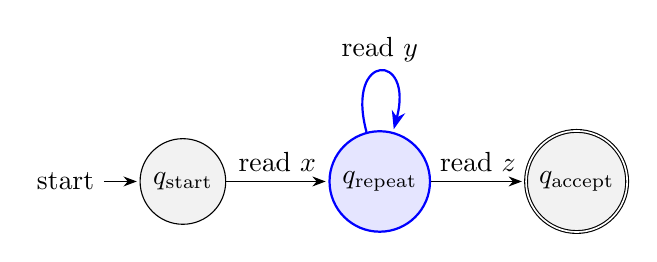
\begin{tikzpicture}[
  ->,>=Stealth,shorten >=1pt,
  node distance=2.5cm,
  every state/.style={minimum size=8mm,fill=black!5}
]
  \node[state,initial] (q0) {$q_{\mathrm{start}}$};
  \node[state,fill=blue!10,draw=blue,thick,right of=q0] (q)
       {$q_{\mathrm{repeat}}$};
  \node[state,accepting,right of=q] (f) {$q_{\mathrm{accept}}$};

  \path
    (q0) edge node[above] {read $x$} (q)
    (q) edge[loop above,thick,blue] node[black] {read $y$} ()
    (q) edge node[above] {read $z$} (f);
\end{tikzpicture}
\end{center}
\end{frame}

%------------------------------------------------
\begin{frame}{Once a Loop Exists, It Can Be Pumped}
Because $y$ starts and ends at the same state, the DFA cannot distinguish
between traversing that loop once, twice, three times, or not at all.

If it accepts
\[
xyz,
\]
it must also accept
\[
xz,\qquad xyyz,\qquad xyyyz,\qquad\ldots
\]

Equivalently, it must accept
\[
xy^iz
\qquad\text{for every }i\geq 0.
\]

\begin{block}{The idea behind every proof}
Choose a string for which changing only the looped part destroys the
property defining the language.
\end{block}
\end{frame}

%================================================
\section{2. The Pumping Lemma and Its Proof}

%------------------------------------------------
\begin{frame}{The Pumping Lemma for Regular Languages}
\begin{block}{Pumping Lemma}
If $A$ is regular, then there exists an integer $p\geq 1$ such that every
string $s\in A$ with $|s|\geq p$ can be written as
\[
s=xyz
\]
so that
\begin{enumerate}
    \item $xy^iz\in A$ for every $i\geq 0$,
    \item $|y|>0$, and
    \item $|xy|\leq p$.
\end{enumerate}
\end{block}

\begin{itemize}
    \item $|y|>0$: the loop must consume at least one symbol.
    \item $|xy|\leq p$: a repeated state is guaranteed within the first
          $p$ symbols.
\end{itemize}
\end{frame}

%------------------------------------------------
\begin{frame}{Formal Proof: Finding the Loop}
\footnotesize
Because $A$ is regular, some DFA
\[
M=(Q,\Sigma,\delta,q_0,F)
\]
recognizes $A$. Let
\[
p=|Q|.
\]

Take any string
\[
s=a_1a_2\cdots a_n\in A,
\qquad n\geq p.
\]
For $0\leq r\leq n$, let
\[
q_r=\delta^*(q_0,a_1a_2\cdots a_r)
\]
be the state reached after reading the first $r$ symbols.

Among
\[
q_0,q_1,\ldots,q_p,
\]
there are $p+1$ state visits but only $p$ possible states. Therefore,
there exist indices
\[
0\leq j<k\leq p
\]
such that
\[
q_j=q_k.
\]
\end{frame}

%------------------------------------------------
\begin{frame}{Formal Proof: Defining $x$, $y$, and $z$}
\footnotesize
Define
\[
x=a_1\cdots a_j,
\qquad
y=a_{j+1}\cdots a_k,
\qquad
z=a_{k+1}\cdots a_n.
\]
Then
\[
s=xyz.
\]
Moreover,
\[
|y|=k-j>0
\]
and
\[
|xy|=k\leq p.
\]

Since $q_j=q_k$, reading $y$ from $q_j$ returns the DFA to $q_j$:
\[
\delta^*(q_j,y)=q_j.
\]
Hence, for every $i\geq 0$,
\[
\delta^*(q_j,y^i)=q_j.
\]
Therefore,
\[
\delta^*(q_0,xy^iz)
=
\delta^*(q_j,y^iz)
=
\delta^*(q_j,z)
=
\delta^*(q_0,xyz)\in F.
\]
Thus $xy^iz\in A$ for every $i\geq 0$. \hfill $\blacksquare$
\end{frame}

%------------------------------------------------
\begin{frame}{What the Proof Actually Established}
The proof did not merely say that long strings ``probably'' contain a
repeatable part.

It constructed a number
\[
p=|Q|
\]
with the following guarantee:

\begin{center}
For every accepted string of length at least $p$,\\
there is at least one legal split whose middle part is a DFA loop.
\end{center}

\begin{alertblock}{Important limitation}
The Pumping Lemma gives a necessary condition for regularity, not a
sufficient one. Successfully pumping some chosen strings does not prove
that a language is regular.
\end{alertblock}
\end{frame}

%================================================
\section{3. Why Negation Creates the Adversary Game}

%------------------------------------------------
\begin{frame}{The Lemma as a Logical Statement}
Ignoring the side conditions for a moment, the pumping property has the
quantifier pattern
\[
\exists p\;
\forall s\;
\exists x,y,z\;
\forall i\geq 0.
\]

More precisely,
\[
\exists p\geq 1\;\forall s:
\Bigl(s\in A\land |s|\geq p\Bigr)
\Longrightarrow
\]
\[
\exists x,y,z:
\left[
\begin{array}{c}
 s=xyz,\ |y|>0,\ |xy|\leq p,\\[0.2em]
 \text{and }xy^iz\in A\text{ for every }i\geq 0
\end{array}
\right].
\]

Each quantifier identifies who gets to choose the next object.
\end{frame}

%------------------------------------------------
\begin{frame}{Negating the Pumping Property}
\small
Negation reverses every quantifier:
\[
\neg\exists=\forall,
\qquad
\neg\forall=\exists.
\]
It also changes
\[
xy^iz\in A
\quad\text{into}\quad
xy^iz\notin A.
\]

Thus, failure of the pumping property means
\[
\forall p\geq 1\;\exists s:
\qquad s\in A\quad\text{and}\quad |s|\geq p,
\]
such that
\[
\forall x,y,z,
\]
if
\[
s=xyz,
\qquad |y|>0,
\qquad |xy|\leq p,
\]
then
\[
\exists i\geq 0
\quad\text{for which}\quad
xy^iz\notin A.
\]
\end{frame}

%------------------------------------------------
\begin{frame}{Why This Proves Nonregularity}
The Pumping Lemma is an implication:
\[
A\text{ regular}
\Longrightarrow
A\text{ has the pumping property}.
\]

Its contrapositive is
\[
A\text{ does not have the pumping property}
\Longrightarrow
A\text{ is not regular}.
\]

Therefore, our task is not to inspect every possible DFA. Instead, we
show that no pumping length $p$ can satisfy the lemma.

\begin{block}{The strategic consequence}
For every proposed $p$, we produce one long string that defeats every
legal decomposition.
\end{block}
\end{frame}

%------------------------------------------------
\begin{frame}{How the Quantifiers Become Players}
\small
\renewcommand{\arraystretch}{1.35}
\begin{center}
\begin{tabular}{p{2.1cm}p{3.1cm}p{7.1cm}}
\toprule
\textbf{Quantifier} & \textbf{Player} & \textbf{Meaning} \\
\midrule
$\forall p$ & \Demon & The argument must work for any pumping length offered. \\
$\exists s$ & \Me & After seeing $p$, I choose a carefully designed string. \\
$\forall x,y,z$ & \Demon & The Demon may choose any split satisfying the rules. \\
$\exists i$ & \Me & After understanding the split, I choose a pump count that breaks membership. \\
\bottomrule
\end{tabular}
\end{center}

\begin{alertblock}{Why the adversary interpretation is exact}
The game is not merely a metaphor. It is the negated quantifier order of
the Pumping Lemma written as a sequence of choices.
\end{alertblock}
\end{frame}

%================================================
\section{4. Demon vs. Me}

%------------------------------------------------
\begin{frame}{The Pumping Lemma Game}
\small
Imagine that the \Demon{} insists that a suspicious language $L$ is regular.

\begin{enumerate}
    \item \Demon{} claims:
    \[
    L\text{ is regular.}
    \]

    \item \Demon{} gives me the pumping length:
    \[
    p\geq 1.
    \]

    \item Poor \Me{} chooses a string:
    \[
    s\in L,
    \qquad |s|\geq p.
    \]

    \item \Demon{} splits it as $s=xyz$, but must obey
    \[
    |y|>0,
    \qquad |xy|\leq p.
    \]

    \item I choose some $i\geq 0$ and force
    \[
    xy^iz\notin L.
    \]
\end{enumerate}

\begin{block}{YAY!}
The Demon fails to satisfy the Pumping Lemma. Therefore, $L$ is not regular.
\end{block}
\end{frame}

%------------------------------------------------
\begin{frame}{What Each Player Controls}
\scriptsize
\renewcommand{\arraystretch}{1.35}
\begin{center}
\begin{tabular}{p{2.5cm}p{4.4cm}p{6.1cm}}
\toprule
\textbf{Player} & \textbf{Chooses} & \textbf{What the choice means} \\
\midrule
\Demon & The pumping length $p$ & We cannot assume a convenient value such as $p=5$. \\
\Me & A long string $s\in L$ & The string should contain a vulnerable region determined by $p$. \\
\Demon & A valid split $s=xyz$ & We may not choose $y$ ourselves. \\
\Me & A pumping value $i$ & The selected $i$ must break membership for every valid split. \\
\bottomrule
\end{tabular}
\end{center}

\begin{alertblock}{The most common mistake}
Writing ``choose $y=0$'' gives \Me{} a move that belongs to the Demon.
We may only prove that every legal $y$ must have some restricted form.
\end{alertblock}
\end{frame}

%================================================
\section{5. The Reusable Victory Script}

%------------------------------------------------
\begin{frame}{The Five-Move Victory Script}
\small
Every correct proof can be organized into the following five moves.

\begin{enumerate}
    \item \textbf{Accept the challenge.}
          Assume, for contradiction, that $L$ is regular.

    \item \textbf{Receive the Demon's number.}
          Let $p$ be the pumping length.

    \item \textbf{Choose the battlefield.}
          Select a string
          \[
          s\in L,
          \qquad |s|\geq p,
          \]
          written in terms of $p$.

    \item \textbf{Trap the Demon's loop.}
          For an arbitrary legal split $s=xyz$, use
          \[
          |xy|\leq p,
          \qquad |y|>0
          \]
          to determine every possible form of $y$.

    \item \textbf{Pump and celebrate.}
          Choose $i\geq 0$ and prove $xy^iz\notin L$.
\end{enumerate}
\end{frame}

%------------------------------------------------
\begin{frame}{The Whole Strategy in One Line}
\small
\begin{center}
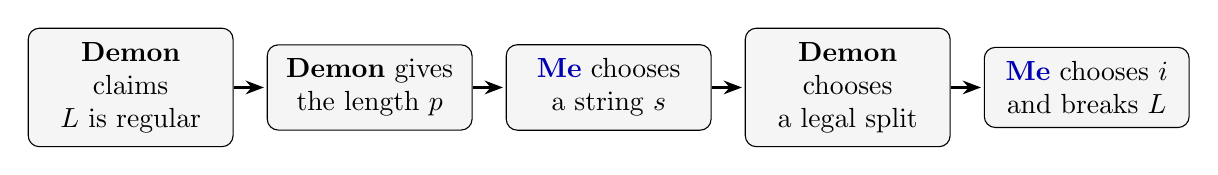
\begin{tikzpicture}[
  node distance=0.42cm,
  every node/.style={align=center},
  boxstep/.style={draw,rounded corners,fill=black!4,inner sep=5pt,text width=2.25cm},
  arr/.style={->,thick}
]
\node[boxstep] (a) {\Demon{} claims\\$L$ is regular};
\node[boxstep,right=of a] (b) {\Demon{} gives\\the length $p$};
\node[boxstep,right=of b] (c) {\Me{} chooses\\a string $s$};
\node[boxstep,right=of c] (d) {\Demon{} chooses\\a legal split};
\node[boxstep,right=of d] (e) {\Me{} chooses $i$\\and breaks $L$};
\draw[arr] (a)--(b);
\draw[arr] (b)--(c);
\draw[arr] (c)--(d);
\draw[arr] (d)--(e);
\end{tikzpicture}
\end{center}

\vspace{0.8em}
\begin{block}{Victory condition}
The rules must trap every legal $y$ tightly enough that some pumping
choice forces $xy^iz\notin L$. Then the Demon loses: \alert{\textbf{YAY!}}
\end{block}
\end{frame}

%================================================
\section{6. Five Battles with the Demon}

%------------------------------------------------
\begin{frame}{Battle 1: Matching Two Blocks}
\small
\[
L_1=\{0^n1^n\mid n\geq 0\}.
\]

\begin{enumerate}
    \item \Demon{} claims that $L_1$ is regular.
    \item \Demon{} gives the pumping length $p$.
    \item Poor \Me{} chooses
    \[
    s=0^p1^p.
    \]
    Clearly, $s\in L_1$ and $|s|=2p\geq p$.
    \item \Demon{} chooses any legal split $s=xyz$.
          Since $|xy|\leq p$, both $x$ and $y$ lie inside the first
          block of $0$s. Since $|y|>0$,
    \[
    y=0^k
    \qquad\text{for some }1\leq k\leq p.
    \]
\end{enumerate}
\end{frame}

%------------------------------------------------
\begin{frame}{Battle 1: I Remove the Loop}
\small
\begin{enumerate}
    \setcounter{enumi}{4}
    \item I choose $i=0$. Then
    \[
    xy^0z=xz=0^{p-k}1^p.
    \]
    The pumped string contains $p-k$ zeros and $p$ ones.

    Since $k>0$,
    \[
    p-k\neq p.
    \]
    Therefore,
    \[
    xz\notin L_1.
    \]
\end{enumerate}

\begin{block}{YAY!}
The Demon's split was arbitrary, yet pumping down always breaks equality.
Thus, $L_1$ is not regular.
\end{block}
\end{frame}

%------------------------------------------------
\begin{frame}{Battle 2: Palindromes}
\small
\[
L_2=\{w\in\{a,b\}^*\mid w=w^R\}.
\]

\begin{enumerate}
    \item \Demon{} claims that $L_2$ is regular.
    \item \Demon{} gives the pumping length $p$.
    \item Poor \Me{} chooses
    \[
    s=a^pba^p.
    \]
    This is a palindrome, and $|s|=2p+1\geq p$.
    \item \Demon{} chooses any legal split $s=xyz$.
          The rule $|xy|\leq p$ traps $y$ inside the first block of $a$s:
    \[
    y=a^k
    \qquad\text{for some }1\leq k\leq p.
    \]
\end{enumerate}
\end{frame}

%------------------------------------------------
\begin{frame}{Battle 2: I Break the Mirror}
\small
\begin{enumerate}
    \setcounter{enumi}{4}
    \item I choose $i=0$. Then
    \[
    xy^0z=a^{p-k}ba^p.
    \]
    There are $p-k$ copies of $a$ to the left of the central $b$, but
    $p$ copies to its right.

    Since $k>0$, the two sides do not match. Therefore,
    \[
    xy^0z\notin L_2.
    \]
\end{enumerate}

\begin{block}{YAY!}
Pumping changes only the left half, so the string loses its symmetry.
Thus, $L_2$ is not regular.
\end{block}
\end{frame}

%------------------------------------------------
\begin{frame}{Battle 3: Synchronizing Three Blocks}
\small
\[
L_3=\{a^nb^nc^n\mid n\geq 0\}.
\]

\begin{enumerate}
    \item \Demon{} claims that $L_3$ is regular.
    \item \Demon{} gives the pumping length $p$.
    \item Poor \Me{} chooses
    \[
    s=a^pb^pc^p.
    \]
    Clearly, $s\in L_3$ and $|s|=3p\geq p$.
    \item \Demon{} chooses any legal split $s=xyz$.
          Since $|xy|\leq p$, the loop is trapped inside the first block:
    \[
    y=a^k
    \qquad\text{for some }1\leq k\leq p.
    \]
\end{enumerate}
\end{frame}

%------------------------------------------------
\begin{frame}{Battle 3: I Change Only One Counter}
\small
\begin{enumerate}
    \setcounter{enumi}{4}
    \item I choose $i=2$. Then
    \[
    xy^2z=a^{p+k}b^pc^p.
    \]
    The three block lengths are now
    \[
    p+k,\qquad p,\qquad p.
    \]
    Since $k>0$, they are not all equal. Hence
    \[
    xy^2z\notin L_3.
    \]
\end{enumerate}

\begin{block}{YAY!}
The Demon can pump only the first block; the other two remain unchanged.
Thus, $L_3$ is not regular.
\end{block}
\end{frame}

%------------------------------------------------
\begin{frame}{Battle 4: Copying Across a Separator}
\small
Let
\[
\Sigma=\{0,1,\#\},
\qquad
L_4=\{w\#w\mid w\in\{0,1\}^*\}.
\]

\begin{enumerate}
    \item \Demon{} claims that $L_4$ is regular.
    \item \Demon{} gives the pumping length $p$.
    \item Poor \Me{} chooses
    \[
    s=0^p1\#0^p1.
    \]
    The same word $0^p1$ occurs on both sides, so $s\in L_4$.
    \item For every legal split, $|xy|\leq p$ traps $y$ in the first
          block of zeros:
    \[
    y=0^k,
    \qquad 1\leq k\leq p.
    \]
\end{enumerate}
\end{frame}

%------------------------------------------------
\begin{frame}{Battle 4: I Edit Only the First Copy}
\small
\begin{enumerate}
    \setcounter{enumi}{4}
    \item I choose $i=0$. Then
    \[
    xy^0z=0^{p-k}1\#0^p1.
    \]
    The word before $\#$ is $0^{p-k}1$, whereas the word after $\#$ is
    still $0^p1$.

    Since $k>0$, the two words differ. Therefore,
    \[
    xy^0z\notin L_4.
    \]
\end{enumerate}

\begin{block}{YAY!}
Pumping edits the first copy while leaving the second copy untouched.
Thus, $L_4$ is not regular.
\end{block}
\end{frame}

%------------------------------------------------
\begin{frame}{Battle 5: Unary Strings of Square Length}
\small
\[
L_5=\{a^{n^2}\mid n\geq 0\}.
\]

\begin{enumerate}
    \item \Demon{} claims that $L_5$ is regular.
    \item \Demon{} gives the pumping length $p\geq 1$.
    \item Poor \Me{} chooses
    \[
    s=a^{p^2}.
    \]
    Since $p^2$ is a square, $s\in L_5$, and $|s|=p^2\geq p$.
    \item Every legal split has
    \[
    y=a^k
    \qquad\text{for some }1\leq k\leq p.
    \]
\end{enumerate}
\end{frame}

%------------------------------------------------
\begin{frame}{Battle 5: I Land Between Two Squares}
\small
\begin{enumerate}
    \setcounter{enumi}{4}
    \item I choose $i=2$. The pumped string has length
    \[
    |xy^2z|=p^2+k.
    \]
    Since $1\leq k\leq p$,
    \[
    p^2<p^2+k\leq p^2+p<(p+1)^2.
    \]
    Thus, $p^2+k$ lies strictly between the consecutive squares
    $p^2$ and $(p+1)^2$.

    Therefore,
    \[
    xy^2z\notin L_5.
    \]
\end{enumerate}

\begin{block}{YAY!}
The pumped length is not a perfect square. Thus, $L_5$ is not regular.
\end{block}
\end{frame}

%------------------------------------------------
\begin{frame}{What the Five Battles Teach Us}
\small
\begin{center}
\begin{tabular}{lll}
\toprule
\textbf{Language type} & \textbf{What must be remembered} & \textbf{What pumping breaks} \\
\midrule
$0^n1^n$ & one unbounded count & equality of two blocks \\
Palindromes & distant symbols & left--right symmetry \\
$a^nb^nc^n$ & three synchronized counts & equality of three blocks \\
$w\#w$ & an entire word & exact copying \\
$a^{n^2}$ & special accepted lengths & arithmetic spacing \\
\bottomrule
\end{tabular}
\end{center}

\vspace{0.7em}
Although the languages look different, each victory follows the same pattern:
\[
\text{claim}\to p\to s\to\text{trap }y\to\text{pump}\to\text{contradiction}.
\]
\end{frame}

%------------------------------------------------
\begin{frame}{Checklist Before Declaring Victory}
When checking a proof, ask:

\begin{enumerate}
    \item Did I assume regularity only for contradiction?
    \item Did I let the Demon choose an arbitrary pumping length $p$?
    \item Did I choose $s$ using $p$?
    \item Did I verify both $s\in L$ and $|s|\geq p$?
    \item Did I analyze every legal split rather than selecting $y$ myself?
    \item Did I use $|xy|\leq p$ and $|y|>0$ explicitly?
    \item Did I choose an $i$ and prove that $xy^iz\notin L$?
\end{enumerate}
\end{frame}

%================================================
\section{7. When Pumping Is Tedious: Closure Traps}

%------------------------------------------------
\begin{frame}{A Different Way to Defeat the Demon}
Sometimes the language is nonregular, but a direct pumping proof gives
the Demon too many annoying cases.

Instead, suppose the language is regular and combine it with languages
already known to be regular.

Because regular languages are closed under operations such as
\[
\cup,\quad \cap,\quad \setminus,\quad \overline{(\cdot)},\quad
\text{reversal},\quad\text{and homomorphism},
\]
the result would also have to be regular.

\begin{block}{Closure trap}
Transform the suspicious language into a known nonregular language.
The contradiction defeats the original regularity claim.
\end{block}
\end{frame}

%------------------------------------------------
\begin{frame}{Closure Trap 1: Unequal Block Lengths}
\small
Consider
\[
L_{\neq}=\{0^m1^n\mid m,n\geq 0,\ m\neq n\}.
\]

The Demon claims that $L_{\neq}$ is regular.

\begin{itemize}
    \item The language $R=0^*1^*$ is regular.
    \item Regular languages are closed under difference.
    \item Therefore, $R\setminus L_{\neq}$ would be regular.
    \item But
    \[
    R\setminus L_{\neq}
    =\{0^n1^n\mid n\geq 0\},
    \]
    which is not regular.
\end{itemize}

\begin{block}{YAY!}
The closure trap exposes the hidden equality language. Therefore,
$L_{\neq}$ is not regular.
\end{block}
\end{frame}

%------------------------------------------------
\begin{frame}{Closure Trap 2: More Ones Than Zeros}
\footnotesize
Consider
\[
L_{<}=\{0^m1^n\mid m<n\}.
\]
Suppose the Demon claims that $L_{<}$ is regular.

\begin{itemize}
    \item Reverse every string, then apply the homomorphism
    \[
    h(0)=1,
    \qquad h(1)=0.
    \]
    Closure under reversal and homomorphism would make
    \[
    L_{>}=\{0^m1^n\mid m>n\}
    \]
    regular.
    \item Hence $L_{<}\cup L_{>}=L_{\neq}$ would be regular.
    \item Therefore,
    \[
    0^*1^*\setminus(L_{<}\cup L_{>})
    =\{0^n1^n\mid n\geq 0\}
    \]
    would also be regular.
\end{itemize}

Contradiction. Thus, $L_{<}$ is not regular.
\end{frame}

%------------------------------------------------
\begin{frame}{Closure Trap 3: Equal Numbers in Any Order}
\small
Consider
\[
E=\{w\in\{0,1\}^*\mid \#_0(w)=\#_1(w)\}.
\]
Suppose the Demon claims that $E$ is regular.

\begin{itemize}
    \item The language $0^*1^*$ is regular.
    \item Regular languages are closed under intersection.
    \item Hence $E\cap 0^*1^*$ would be regular.
    \item However,
    \[
    E\cap 0^*1^*
    =\{0^n1^n\mid n\geq 0\},
    \]
    which is not regular.
\end{itemize}

\begin{block}{YAY!}
Intersection removes all distracting arrangements and reveals the
nonregular core. Therefore, $E$ is not regular.
\end{block}
\end{frame}

%================================================
\section{8. Compact Practice Examples}

%------------------------------------------------
\begin{frame}{More Battles with the Demon I}
\scriptsize
\renewcommand{\arraystretch}{1.34}
\setlength{\tabcolsep}{3pt}
\begin{center}
\begin{tabular}{p{3.0cm}p{2.4cm}p{2.3cm}p{5.3cm}}
\toprule
\textbf{Language} &
\textbf{My string $s$} &
\textbf{The rules force} &
\textbf{My winning move} \\
\midrule
$\{a^{n+1}b^n\mid n\geq 0\}$ &
$a^{p+1}b^p$ &
$y=a^k$, $k>0$ &
Choose $i=0$. Then $a^{p+1-k}b^p$ no longer has exactly one more $a$ than $b$. \\
\addlinespace
$\{a^mb^n\mid m>n\}$ &
$a^{p+1}b^p$ &
$y=a^k$, $k>0$ &
Choose $i=0$. Since $p+1-k\leq p$, the number of $a$s is no longer greater. \\
\addlinespace
$\{a^nb^{2n}\mid n\geq 0\}$ &
$a^pb^{2p}$ &
$y=a^k$, $k>0$ &
Choose $i=0$. The counts become $p-k$ and $2p$, but $2p\neq2(p-k)$. \\
\addlinespace
$\{a^mb^nc^{m+n}\mid m,n\geq 0\}$ &
$a^pb^pc^{2p}$ &
$y=a^k$, $k>0$ &
Choose $i=0$. The first two blocks total $2p-k$, while the last block remains $2p$. \\
\addlinespace
$\{a^ib^jc^k\mid i=j\text{ or }j=k\}$ &
$a^pb^pc^{p+1}$ &
$y=a^r$, $r>0$ &
Choose $i=0$. Now $p-r\neq p$ and $p\neq p+1$, so neither equality holds. \\
\bottomrule
\end{tabular}
\end{center}
\end{frame}

%------------------------------------------------
\begin{frame}{More Battles with the Demon II}
\scriptsize
\renewcommand{\arraystretch}{1.34}
\setlength{\tabcolsep}{3pt}
\begin{center}
\begin{tabular}{p{3.0cm}p{2.5cm}p{2.2cm}p{5.3cm}}
\toprule
\textbf{Language} &
\textbf{My string $s$} &
\textbf{The rules force} &
\textbf{My winning move} \\
\midrule
$\{u\#v\mid |u|=|v|\}$ &
$0^p\#1^p$ &
$y=0^k$, $k>0$ &
Choose $i=0$. The two sides now have lengths $p-k$ and $p$. \\
\addlinespace
$\{a^q\mid q\text{ is prime}\}$ &
$a^q$, prime $q>p$ &
$y=a^k$, $1\leq k\leq p$ &
Choose $i=q+1$. The new length is $q+qk=q(k+1)$, which is composite. \\
\addlinespace
$\{a^{2^n}\mid n\geq 0\}$ &
$a^{2^m}$, $2^m>p$ &
$y=a^k$, $1\leq k\leq p$ &
Choose $i=2$. Then $2^m<2^m+k<2^{m+1}$, so the length is not a power of two. \\
\addlinespace
$\{a^mb^n\mid m=n\text{ or }m=2n\}$ &
$a^pb^p$ &
$y=a^k$, $k>0$ &
Choose $i=0$. The new $a$-count $p-k$ is neither $p$ nor $2p$. \\
\addlinespace
$\{a^mb^{m+n}c^n\mid m,n\geq 0\}$ &
$a^pb^{2p}c^p$ &
$y=a^k$, $k>0$ &
Choose $i=0$. The outer blocks total $2p-k$, but the middle block still has length $2p$. \\
\bottomrule
\end{tabular}
\end{center}
\end{frame}

%------------------------------------------------
\begin{frame}{Problems to Try at Home}
\small
For each language, decide whether a direct Demon game or a closure trap
is the cleaner proof.

\begin{itemize}
    \item $L_1=\{0^m1^n\mid m\neq n\}$.
    \item $L_2=\{0^m1^n\mid \gcd(m,n)=1\}$.
    \item $L_3=\{0^m1^n\mid m\mid n,\ m,n\geq 1\}$.
    \item $L_4=\{(ab)^nc^n\mid n\geq 0\}$.
    \item $L_5=\{a^{n!}\mid n\geq 1\}$.
    \item $L_6=\{a^{F_n}\mid n\geq 0\}$, where $F_n$ is the $n$th Fibonacci number.
    \item $L_7$ is the language of correctly balanced parenthesis strings over $\{(,)\}$.
\end{itemize}
\end{frame}

%------------------------------------------------
\begin{frame}{Summary}
\begin{itemize}
    \item \textbf{Graph intuition:} A long DFA computation must revisit a state.
    \item \textbf{Formal proof:} The repeated state produces a nonempty loop $y$ within the first $p$ symbols.
    \item \textbf{Logical foundation:} Negating the lemma changes
    \[
    \exists p\,\forall s\,\exists(x,y,z)\,\forall i
    \]
    into
    \[
    \forall p\,\exists s\,\forall(x,y,z)\,\exists i.
    \]
    \item \textbf{Adversary strategy:} The Demon chooses $p$ and the split; we choose $s$ and $i$.
    \item \textbf{Alternative strategy:} Closure operations can expose a known nonregular language.
\end{itemize}

\vspace{0.8em}
\textit{Next Lecture:} Context-Free Grammars and recursive structure.
\end{frame}

\end{document}
